\documentclass[landscape]{slides}
\usepackage[landscape, margin=2cm]{geometry}
\usepackage{color}
\usepackage{bm}
\usepackage{graphicx}
\usepackage{hyperref}
\graphicspath{ {./img/} {./charts/} }



\title{Show and Tell: Skill Acquisition}
\author{Adam Johnson - me@adamj.eu}
\date{28th August 2013}

\begin{document}

\maketitle

\begin{slide}

    \textcolor{blue}{\Large{Skill Acquisition}}

    \begin{itemize}
        \item I like learning
        \item I like tracking myself
        \item This is me tracking myself learn
    \end{itemize}

\end{slide}

\begin{slide}

    \textcolor{blue}{\Large{The Skill}}

    \begin{itemize}
        \item Something I bet you did today...
        \item and were paid to do it...
        \item and you probably never practiced it...
    \end{itemize}

\end{slide}

\begin{slide}

    \textcolor{blue}{\Large{Typing!}}

    
\includegraphics[height=10cm]{baby-nerd}

\end{slide}


\begin{slide}

    \textcolor{blue}{\Large{Motivation}}

    \begin{itemize}
        \item Extreme fear of RSI
        \item Always \emph{intended} to learn to touchtyping
        \item Wikipedia: ``In the USA, carpal tunnel syndrome results in an average of \$30,000 in lifetime costs''
    \end{itemize}

\end{slide}


\begin{slide}

    \textcolor{blue}{\Large{To business!}}

    \begin{itemize}
        \item Just grab some typing programs
        \item Learn QWERTY the right way!!
    \end{itemize}

\end{slide}


\begin{slide}

    \textcolor{blue}{\Large{Oh no....}}

\end{slide}

\begin{slide}
    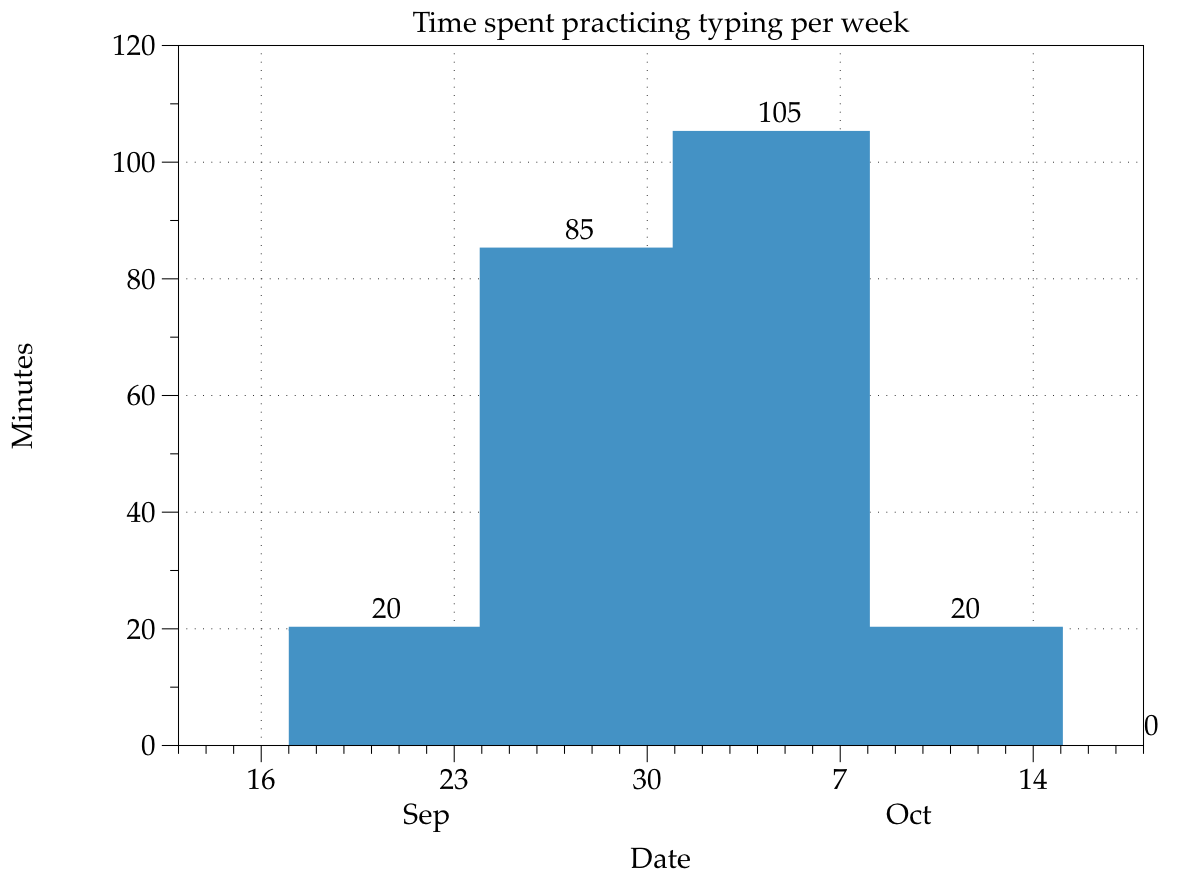
\includegraphics[width=\textwidth]{first-practice}
\end{slide}

\begin{slide}
    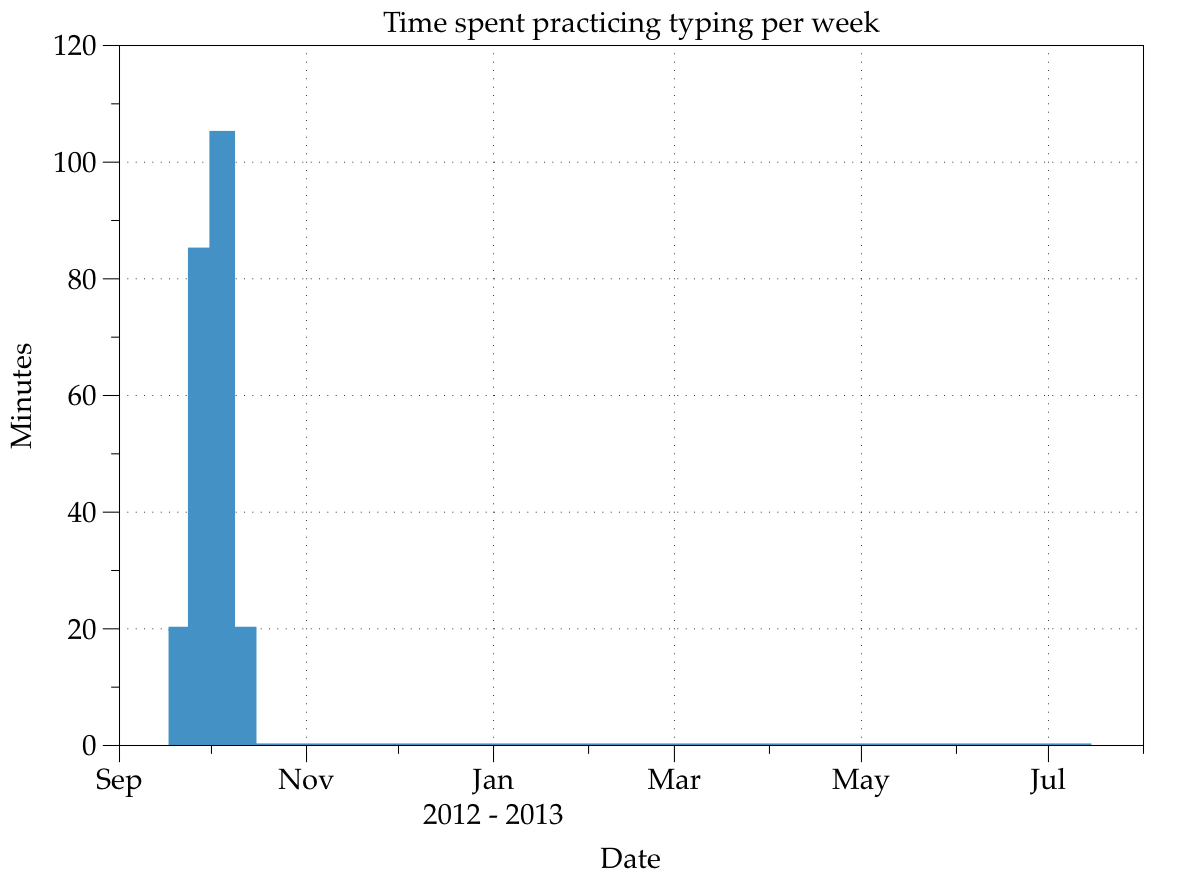
\includegraphics[width=\textwidth]{first-practice-long-tail}
\end{slide}


\begin{slide}

    \textcolor{blue}{\Large{Motivation}}

    \begin{itemize}
        \item Extreme fear of RSI
        \item Always \emph{intended} to learn to touchtyping
        \item Found a book that inspired me
    \end{itemize}

\end{slide}


\begin{slide}

    \textcolor{blue}{\Large{The First 20 Hours}}

    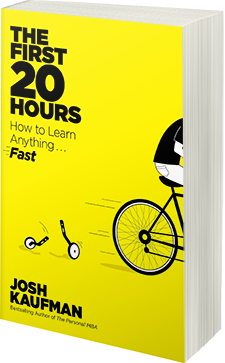
\includegraphics[height=10cm]{first20hours-cover}

    \begin{itemize}
        \item Josh Kaufman
    \end{itemize}

\end{slide}

\begin{slide}

    \textcolor{blue}{\Large{The First 20 Hours}}

    \begin{itemize}
        \item Learning a skill shouldn't take more than 20 hours to get to a good enough standard
        \item A couple chapters of general how-to, then one chapter on each skill he learnt with his method
        \item One of these was touchtyping... with `Colemak'
    \end{itemize}

\end{slide}


\begin{slide}

    \textcolor{blue}{\Large{QWERTY}}

    \centering
    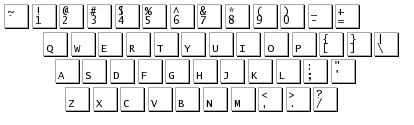
\includegraphics[width=20cm]{qwerty}

    \begin{itemize}
        \item Checkered past...
    \end{itemize}

\end{slide}


\begin{slide}

    \textcolor{blue}{\Large{Colemak}}

    \centering
    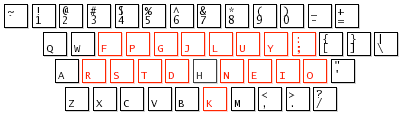
\includegraphics[width=20cm]{colemak-annot}

    \begin{itemize}
        \item Smooth future...
    \end{itemize}

\end{slide}


\begin{slide}
    \textcolor{blue}{\Large{Thank you}}

    \begin{itemize}
        \item Slides on GitHub - \url{http://is.gd/adamIsDaBomb}
        \item Email me - \url{me@adamj.eu}
    \end{itemize}

\end{slide}


\end{document}
